\section{System Management Mode (\gls{smm})}\label{section-smm}
\subsection{Overview}
On IA-32 processors, System Management Mode (\gls{smm}) is a mode of operation which is distinct from the flat model, protected mode operation of the DXE and PEI phases. It is defined as a real-mode environment with 32-bit data access and its activated in effect to an interrupt type or using the System Management Interrupt (\gls{smi}) pin. Note that SMM is OS-transparent mode of operation and is distinct operational mode and also it coexist within and OS runtime.

\begin{figure}[!htbp]
	\centering
	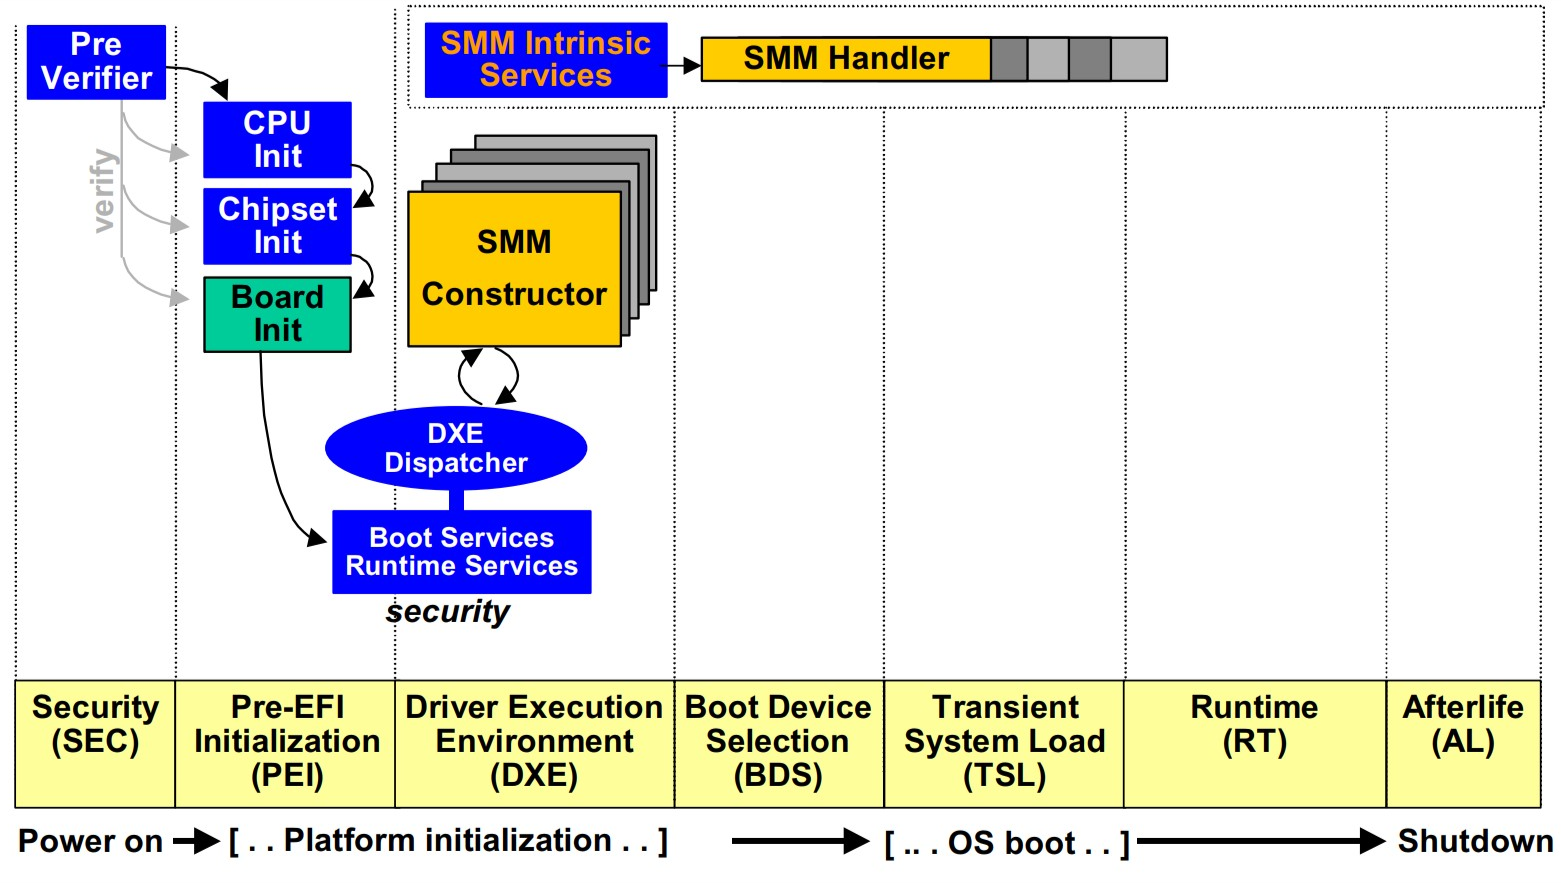
\includegraphics[width=0.9\linewidth]{smm/framework-smm-architecture}
	\caption{SMM Framework Architecture}\label{fig:framework-smm-architecture}
\end{figure}


\subsection{System Management System Table (\gls{smst})}
System Management System Table (\gls{smst}) is core mechanism of SMM handler to pass information and enabling activity.

SMST table provides access to the SMST-based services, known as SMM Services. Driver can only use SMM services while executing within the SMM context. \verb|EFI_SMM_BASE_PROTOCOL.GetSmstLocation()| service used to discover the address of SMST.

SMST is a set of capabilities exported for use by any driver that is loaded into SMRAM. It's akin to the EFI System Table, where it is a fixed set of services and data, by design, and does not acknowledge to the extensibility of an EFI protocol interface.

SMM infrastructure component of Framework provides SMST, which manages:
\begin{itemize}
	\item Dispatching drivers in SMM
	\item Allocations of SMRAM
	\item Transitioning the framework into and out of the respective SMM of the processor
\end{itemize}

\subsection{SMM and Available Services}\label{subsection-smm-available-services}

\subsubsection{SMM Services}\label{subsection-smm-services}
The model of SMM in the Framework will have constraints similar to those of EFI runtime drivers.
Specifically, the dispatch of drivers in SMM will not be able to use core protocol services. There
will be SMST-based services, called SMM Services, that the drivers can access using an SMM
equivalent of the EFI System Table, but the core protocol services will not necessarily be available
during runtime.
Instead, the full collection of EFI Boot Services and EFI Runtime Services are available only
during the driver load or "constructor" phase. This constructor visibility is useful in that the SMM
driver can leverage the rich set of EFI services to do the following:
\begin{itemize}
	\item Marshall interfaces to other EFI services.
	\item Discover EFI protocols that are published by peer SMM drivers during their constructor phases.
\end{itemize}
This design makes the EFI protocol database useful to these drivers while outside of SMM and
during their initial load within SMM.
The SMST-based services that are available include the following:
\begin{itemize}
	\item A minimal, blocking variant of the device I/O protocol
	\item A memory allocator from SMM memory
\end{itemize}
These services are exposed by entries in the System Management System Table (SMST)

\subsubsection{SMM Library (SMLib Services)}\label{subsection-smm-lib}
Additional services in the SMM Library (SMLib) are exposed as conventional EFI protocols that
are located during the constructor phase of the SMM driver in SMM. For example, the status code
equivalent in SMM is simply an EFI protocol whose interface references an SMM-based driver's
service. Other SMM drivers locate this SMM-based status code and can use it during runtime to
emit error or progress information.

\subsection{SMM Drivers}\label{subsection-smm-drivers}
\subsubsection{Loading Drivers into SMM}
Driver loading modal into SMM is that the DXE SMM runtime driver contains a dependency expression that at least have the \verb|EFI_SMM_BASE_PROTOCOL|. This dependency is essential because the DXE runtime driver that is planned for SMM will use the \verb|EFI_SMM_BASE_PROTOCOL| to reload itself into SMM and re-execute its entry point in SMM. Also, other SMM-loaded protocols allowed to be situated in the dependency expression of a given SMM DXE runtime driver. The principle of the DXE Dispatcher, verifying if the GUIDs for the protocols that are exist in the protocol database can then be used to identify if the driver can be loaded. 

Once loaded into SMM, the DXE SMM runtime driver can utilize a very minor set of services. While in its constructor entry point, the driver can use EFI Boot Services as it runs in the boot service space and SMM. In this second entry point in SMM, the driver can do several things:

\begin{itemize}
	\item Register an interface in the conventional protocol database to name the SMM resident interfaces to future-loaded SMM drivers
	\item Register with the SMM infrastructure code for a callback in effect to an SMI pin activation or an SMI based message from outside of SMM Code (i.e. a boot service, runtime agent)
\end{itemize}

After this \textbf{constructor} phase in SMM, the SMM driver should not depend upon any other boot services because the operational mode of execution can migrate away from these services (the \verb|ExitBootServices()| call is asynchronous to calling the SMM infrastructure code). Several EFI Runtime Services can have the bulk of their processing shifted into SMM, and the runtime visible portion would simply be a proxy that uses the \verb|EFI_SMM_BASE_PROTOCOL| to callback into SMM to carry out the services. Having a proxy allows for a model of sharing error handling code, such as flash access services, along with runtime code, such as the EFI Runtime Services \verb|GetVariable()| or \verb|SetVariable()|.

\subsubsection{IA-32 SMM Drivers}
In SMM the IA-32 runtime drivers are not callable because of the \verb|SetVirtualAddress()| action that is performed upon the image. As such, code that needs to be accessible between SMM and EFI runtime needs to migrate into SMM.

\subsubsection{Itanium® Processor Family SMM Drivers}
From Platform Management Interrupt (\gls{pmi}) the runtime drivers for the Itanium® processor family are callable as each is a variant of position-independent code (PIC) runtime driver.

\subsection{SMM Protocols}\label{subsection-smm-protocols}
System Architecture of SMM broke in to below two parts:
\begin{itemize}
	\item SMM Base Protocol - published by a processor and its responsible for: 
		\begin{itemize}
			\item To initialize the state of processor
			\item Registration of the handlers
		\end{itemize}
	\item SMM Access Protocol - interprets the specific enable and locking techniques that an IA-32 memory controller might support during execution in SMM. (Not needed for Itanium® processor family)
\end{itemize}

\subsubsection{SMM Protocols for IA-32}
Figure \ref{fig:published-protocols-for-ia-32-systems} shows the SMM protocols which are published for an IA-32 system.
\begin{figure}[!htbp]
	\centering
	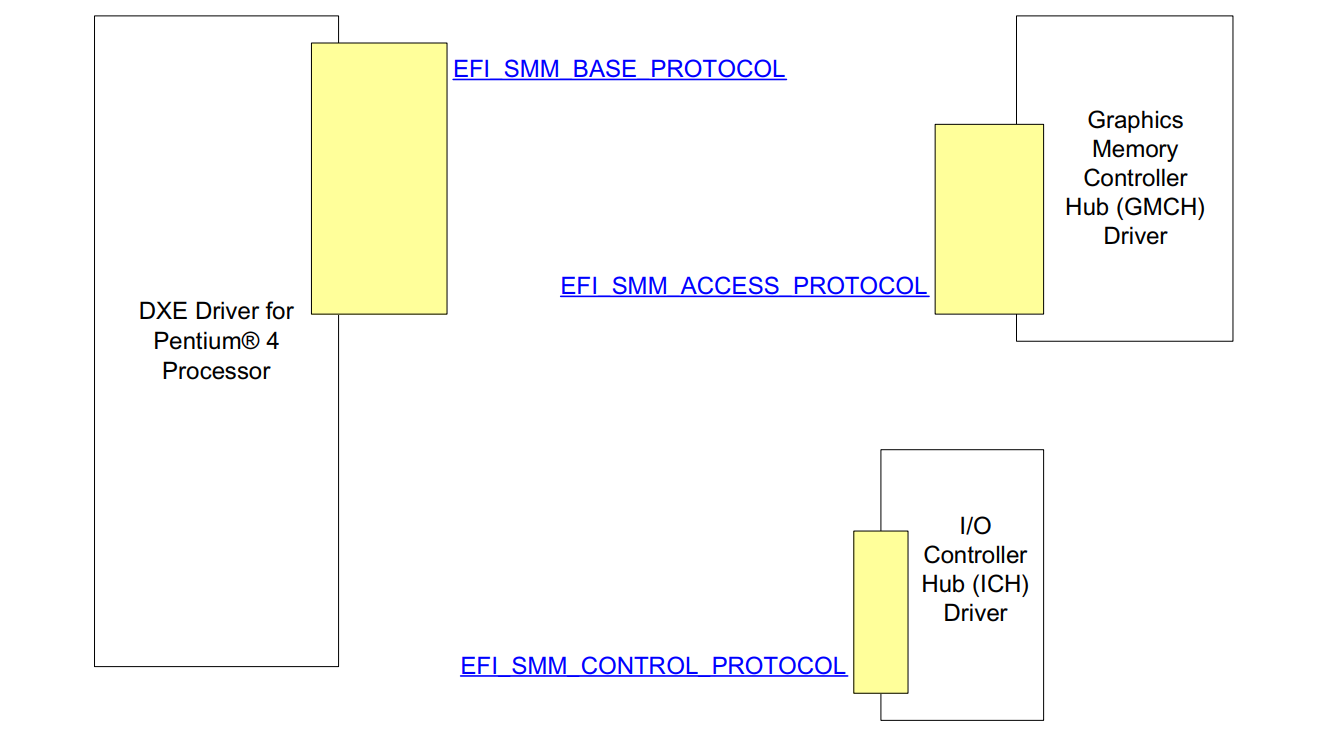
\includegraphics[width=0.9\linewidth]{smm/published-protocols-for-ia-32-systems}
	\caption{Protocols Published for IA-32 Systems}\label{fig:published-protocols-for-ia-32-systems}
\end{figure}

\subsubsection{SMM Protocols for Itanium®-Based Systems}
Figure \ref{fig:published-protocols-for-itanium-systems} shows the SMM protocols which are published for an Itanium®-Based system.
\begin{figure}[!htbp]
	\centering
	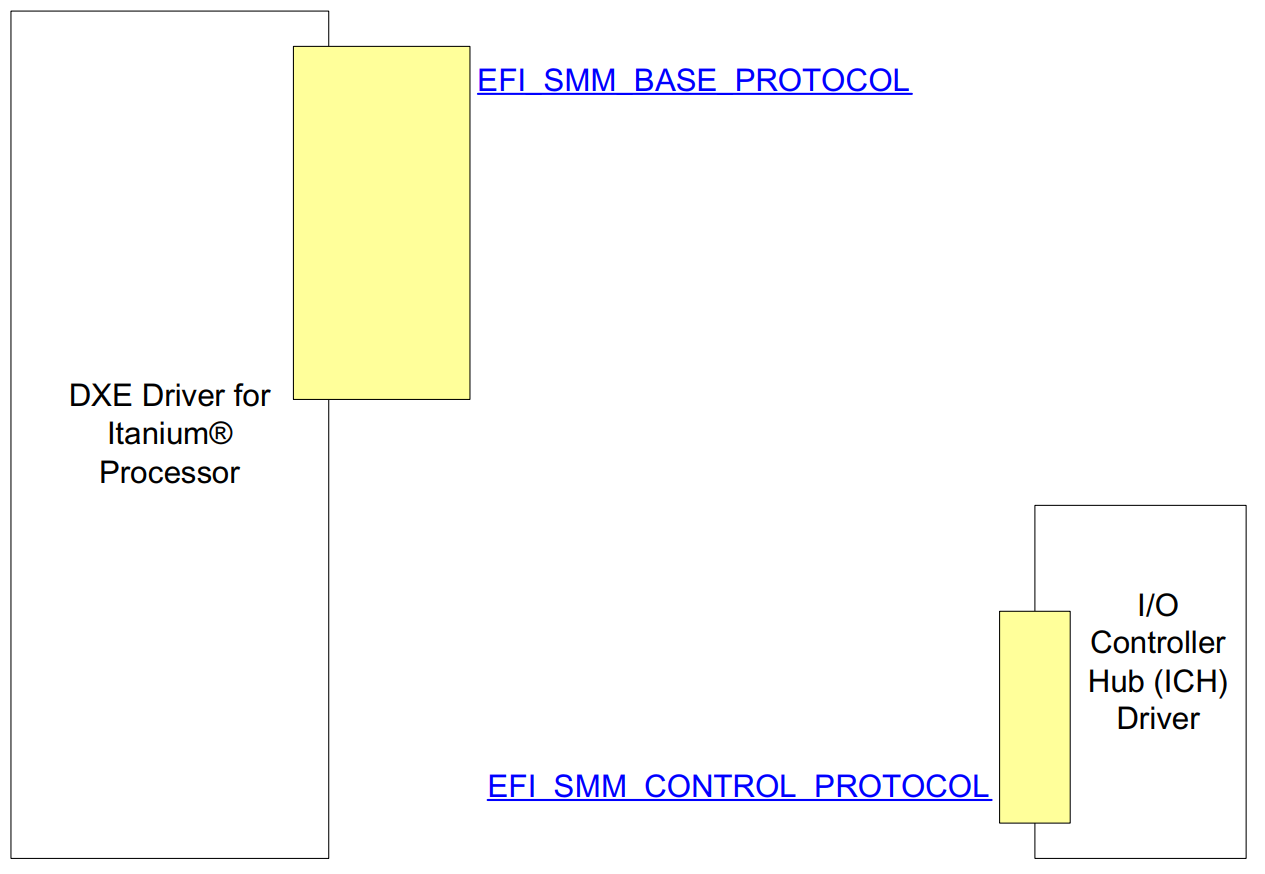
\includegraphics[width=0.9\linewidth]{smm/published-protocols-for-itanium-systems}
	\caption{Protocols Published for Itanium®-Based Systems}\label{fig:published-protocols-for-itanium-systems}
\end{figure}


\subsection{SMM Infrastructure Code and Dispatcher}
SMM Infrastructure Code centers within the SMM Dispatcher. Role of SMM Dispatcher is to hand over the control to the SMM handlers in an orderly manner. SMM Infrastructure Code assists to drive SMM to SMM communication. SMM handlers are PE32+ images that have and image type of \verb|EFI_IMAGE_SUBSYSTEM_EFI_RUNTIME_DRIVER|.

\subsection{Initializing SMM Phase}
The SMM driver for the Framework is essentially a enrollment vehicle for dispatching drivers in response to the:
\begin{itemize}
	\item System Management Interrupts for IA-32
	\item Platform Management Interrupts (PMIs) for Itanium® processor family
\end{itemize}

\subsection{Relation of System Management RAM (SMRAM) to main memory}
Figure \ref{fig:smram-relationship-to-main-memory} shows relationship between SMRAM and main memory in IA-32.

\begin{figure}[!htbp]
	\centering
	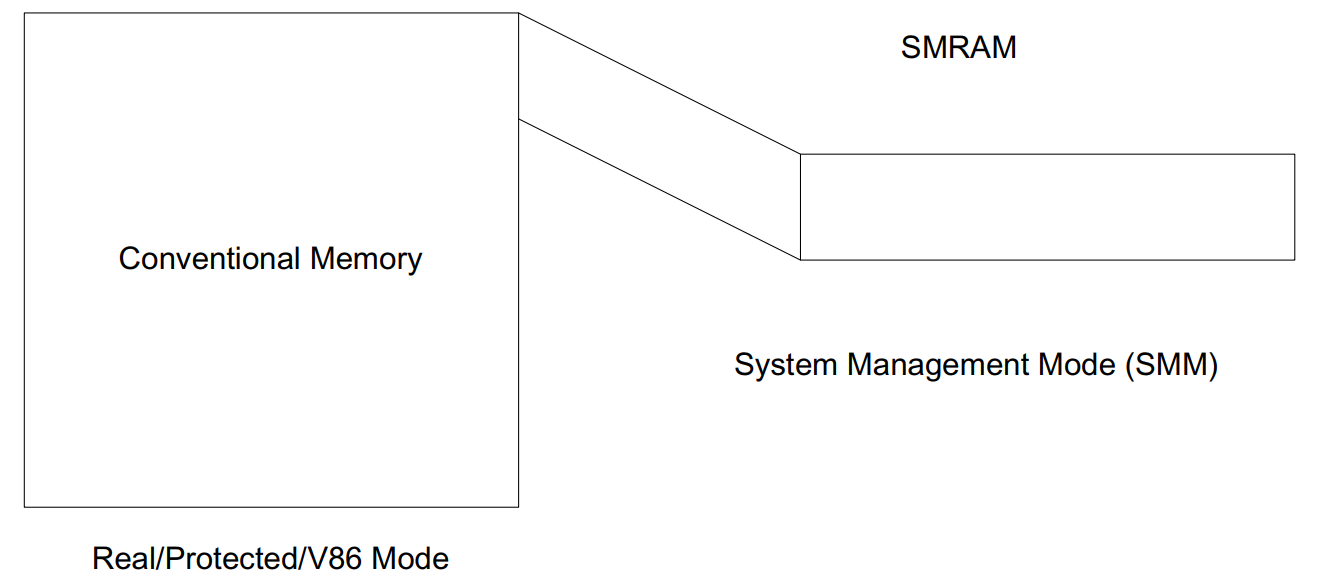
\includegraphics[width=0.9\linewidth]{smm/smram-relationship-to-main-memory}
	\caption{SMRAM relationship to main memory}\label{fig:smram-relationship-to-main-memory}
\end{figure}

\subsection{Processor Execution Mode}\label{subsection-processor-execution-mode}
SMM is entered asynchronously to the main flow of program. SMM was originally designed to be clear to the OS and provides a transparent power management facility. 

Preboot agents are responsible to initiate alternate uses of SMM which are:
\begin{itemize}
	\item Workarounds for chipset errata
	\item Error logging
	\item Platform security
\end{itemize}

A \gls{smi} can be entered by energizing either the SMI logic pin on the baseboard dedicated or using the local APIC.

Itanium® architecture has no separated processor mode for the manageability interruption, but it supports Platform Management Interrupt (\gls{pmi}), which is a maskable interruption. Also, another way to enter PMI is using a message on local Streamlined Advanced Programmable Interrupt Controller (\gls{sapic}).

This architecture describes a mechanism for loading modules of needful code that substantiate the functionality mentioned above. The instantiation of protocol that enables the loading of handler images runs in normal boot-services memory. Only handler need to run in the \gls{smram}.

\subsection{Access to Platform Resources}\label{subsection-access-to-platform-resources}
As a policy outcome, execution of SMM handlers is logically precluded from accessing traditional memory resources. Hence, there is no ease binding technique through a call or trap interface to leverage services in the preempted, non-SMM state.

Besides, SMM Services - the library of service, supports a subset of the core EFI services, i.e. memory allocation, device I/O protocol, and others. Also, SMM driver execution mode has the same structure as the EFI baseline - namely a components that runs in boot services mode and that can perhaps execute in runtime. Another mechanism occurs using an unregister event when \verb|ExitBootServices()| is invoked.



